\chapter[Desenvolvimento e Metodologia]{Desenvolvimento e Metodologia}

\section{Algoritmo}

\subsection{Seleção de Variáveis \textit{Stepwise}}

O algoritmo proposto nesse trabalho é baseado no método de seleção de variáveis \textit{stepwise} 
(\textit{Stepwise Selection}), comumente utilizado em conjunto com modelos de regressão linear. É um método de
\textit{greedy search}, onde, a cada iteração, a variável que apresentar o melhor ganho de performance é 
adicionada ao conjunto de entradas. 

O modelo é construido incrementalmente até que não haja mais melhora de performance ao acrescentar alguma das 
variáveis restantes ou não haja mais variáveis para serem consideradas. O método é descrito em pseudocódigo no 
algoritmo \ref{alg:stepwiseselection}
\\


\begin{algorithm}[H]
    \caption{\textit{Forward Stepwise Selection} (FSS)}
    \KwIn{$variáveis$: lista contendo as variáveis disponíveis;}
    \KwIn{$saídas$: lista contendo as saídas do modelo;}
    \KwOut{$selecionadas$: lista de variáveis relevantes.}
    $selecionadas \gets \{\ \}$ \\
    $melhorErro \gets \infty$ \\
    \Repeat{$variáveis == \{\ \}$ ou (critério de parada)}
    {   
        $melhorVariável \gets NULL$ \\     
        \ForEach{elemento $var$ em $variáveis$}{
            $entradas \gets (var \cup selecionadas)$ \\
            $model \gets ajuste(entradas,saídas)$ \\
            $erro \gets avalia(model,entradas,saídas)$ \\
            \If{$erro <melhorErro$}{
                $melhorErro \gets erro$\\
                $melhorVariável \gets var$ \\     
            }
        }
        $selecionadas \gets (melhorVariável \cup selecionadas)$ \\
        $variáveis \gets (variáveis \setminus \{melhorVariável\})$ \\
    }
    \label{alg:stepwiseselection}
\end{algorithm}

\qquad

Esse algoritmo apresenta uma redução expressiva na quantidade de modelos ajustados em relação ao método da 
seleção do melhor subconjunto, que é um algoritmo de busca exaustiva, onde todas as combinações possíveis das 
variáveis de entrada são testadas. Na primeira iteração, o modelo nulo deve ser ajustado, em seguida, todas as 
$p$ varíaveis devem ser avaliadas e, a cada iteração posterior, uma delas é retirada. Portanto o total de 
modelos ajustados pode ser descrito pela eq. \ref{eq:total_models}

\begin{equation}
    Ajustes = 1 + \sum^{p-1}_{k = 0} (p-k) = 1 + \dfrac{p (p+1)}{2} =  \dfrac{1}{2} (p^2 + p  + 2)
    \label{eq:total_models}
\end{equation}

Porém, ao contrário do método da seleção do melhor subconjunto, não há garantia que o subconjunto determinado é 
a combinação ótima das variáveis \cite[p. 208]{intro_stat_learn}.

Um fator determinante para a eficácia do algoritmo é a escolha da métrica pela qual os modelos serão avaliados. A utilização de uma métrica que considere simplesmente os dados ajustados não é adequada, 
uma vez que, nessa situação, o incremento de uma variável no modelo sempre acarretará em uma melhora no erro de treinamento, porém não necessariamente na capacidade de generalização do modelo.

Algumas técnicas tentam determinar a capacidade de generalização através de informações obtidas com os dados de treinamento, tais como o critério de Informação de Akaike (AIC) ou critério de informação Bayesiano (BIC), porém elas se baseiam no comportamento assintótico, isto é, quando a quantidade de amostras é bastante elevada.

Uma alternativa a essas técnicas é a utilização de validação cruzada, onde o modelo selecionado é aquele que apresenta a melhor performance no conjunto de testes. Dessa maneira, obtém-se diretamente uma estimativa do erro de generalização, além de se assumir menos condições em relação ao modelo e aos dados utilizados. O grande desafio dessa técnica é o custo computacional da validação cruzada que, quando associado ao custo do método de seleção de variáveis \textit{stepwise} pode tornar proibitiva sua implementação.

Em especial, a utilização desse método associada ao \textit{leave-one-out cross-validation} resultaria no ajuste de $\sfrac{1}{2}(p^2+p+2)(N-1)$ modelos, tornando o algoritmo computacionalmente inviável.

\subsection{Método Incremental}

Para minimizar o problema do custo computacional, o método implementado utiliza o resultado apresentado na eq. 
\ref{eq:LOOCV_error} para calcular o erro de validação cruzada sem a necessidade de cálcular $N-1$ modelos de 
regressão linear. Além disso, o cálculo da matriz de aniquilação é realizado de maneira incremental, conforme 
deduzido na eq. \ref{eq:inc_matrix_iterativa}.

O algoritmo \ref{alg:stepwiseselection} é então modificado para realizar o cálculo incremental, utilizando 
LOOCV como métrica para seleção dos das variáveis e atualização incremental do modelo.

\qquad

\begin{algorithm}[H]
    \caption{\textit{Forward Stepwise Incremental Selection}}
    \KwIn{$variáveis$: lista contendo as variáveis disponíveis;}
    \KwIn{$saídas$: lista contendo as saídas do modelo;}
    \KwOut{$selecionadas$: lista de variáveis relevantes.}
    
    $selecionadas \gets \{\ \}$ \\
    $melhorErro \gets \infty$ \\
    $M \gets I_N$ \\

    \Repeat{$variáveis == \{\ \}$ ou (critério de parada)}
    { 
        $melhorVariável \gets NULL$ \\
        \ForEach{elemento $var$ em $variáveis$}{
            $M' \gets ajusteIncremental(M,var)$ \\
            $erro  \gets erroLOOCV(M,saídas)$ \\
            \If{$erro <melhorErro$}{
                $melhorErro \gets erro$\\
                $melhorVariável \gets var$ \\                
                $melhorM \gets M' $  \\
            }
        }
        $M \gets melhorM $ \\
        $selecionadas \gets (melhorVariável \cup selecionadas)$ \\
        $variáveis \gets (variáveis \setminus \{melhor_{variável}\})$ \\
    }
    \label{alg:incstepwiseselection}
\end{algorithm}



\section{Testes e Validação}

\subsection{Conjuntos de dados}

Para teste e validação do algoritmo desenvolvido, utilizou-se três bancos de dados conhecidos na literatura, 
especificados na tabela \ref{tbl:datasets}.
\begin{table}[H]
    \caption{Conjuntos de dados utilizados para validação.}
    \centering
    \begin{tabular}{@{}lll@{}}
    \toprule
    Nome                           & Variáveis & Amostras \\ \midrule
    \textit{Forest Fires}          & 12        & 517      \\
    \textit{USA Housing Dataset}   & 80        & 1460     \\
    \textit{Wiscoin Breast Cancer} & 32        & 194      \\ \bottomrule
    \end{tabular}
    \label{tbl:datasets}
\end{table}

\subsubsection{Preprocessamento}

De maneira geral, em um conjunto de amostras, as variáveis apresentam diferentes unidades, magnitudes e escalas, 
isso dificulta a comparação de valores e pode prejudicar o treinamento de modelos. Por isso é comum aplicar uma 
transformação nos dados, de maneira a torna-los comparáveis entre si (\textit{feature scaling}), além de 
facilitar a detecção de \textit{outliers}.

Embora o algoritmo utilizado se baseie em regressões lineares que, em sua forma mais simples, são robustas em 
relação a magnitude das variáveis, a adição do termo de regressão penaliza o crescimento do vetor de parâmetros, 
tornando o modelo sensivel à diferença de magnitudes entre variáveis.

Nesse trabalho, todas as variáveis foram normalizadas, de maneira a se obter entradas e saídas que apresentam 
média nula e desvio padrão unitário. Tal transformação é conhecida como \textit{z-score} (eq. \ref{eq:z-score}).

\begin{equation}
    X_p = \frac{ X_p - \bar{X_p} }{SD(X_p)}
    \label{eq:z-score}
\end{equation}

Além disso, uma variável de entrada com valor unitário foi adicionada posteriormente a cada conjunto de dados, 
permitindo a consideração do termo livre ($w_0$) nos cálculos de maneira transparente.

\subsection{Metodologia de Validação}

Com o intuito de identificar um subconjunto ótimo de variáveis para cada conjunto de dados, o algoritmo 
desenvolvido foi empregado e o erro de validação cruzada, conforme a eq. \ref{eq:LOOCV_error}, foi registrado 
ao final de cada iteração. Dessa maneira é possível analisar o efeito da inclusão de uma nova variável na 
capacidade de generalização do modelo e avaliar até onde é benéfico o aumento de uma nova dimensão.

Além disso, verificou-se a influência do número de amostras e dimensões no modelo. Para isso, o procedimento 
anterior foi repetido em subconjuntos de menos amostras ($50\%$, $33\%$, $25\%$), selecionadas aleatoriamente 
múltiplas vezes. O erro inicial médio de cada um desses experimentos foi deslocado para zero, de maneira a 
permitir a comparação dos resultados em função do aumento do número de dimensões.

% \subsection{Estudo de Caso: \textit{Brazilian Coins}}

% Um estudo mais detalhado foi realizado considerando dados extraídos do conjunto de imagens \textit {Brazilian Coins} \cite{brazilian_coins}. Para esse estudo desenvolveu-se um script em Python que localiza, recorta e redimensiona a região onde se localiza a moeda na imagem original. Um exemplo de imagem original e pós processamento pode ser visto na fig.\ref{fig:coin_extract}.

% \begin{figure}[H]
%     \caption{Extração de uma moeda da imagem}
%     \centering
%     \adjincludegraphics[width=0.8\textwidth,trim={0 {0.15\height} 0 {0.15\height}},clip]{imgs/met/sampleExtraction.png}
%     \legend{Fonte: Própria. Adaptada de \cite{brazilian_coins}}
%     \label{fig:coin_extract}
% \end{figure}

% Em seguida a moeda é dividida em 3 anéis concêntricos e um círculo central. De cada região é extraída a quantidade de quinas (corners). Além disso, a média de cada canal de cores (RGB) na região central e no anel externo são computadas, bem como o total de círculos presentes na moeda. O script desenvolvido se encontra na integra no \textcolor{red}{REFERENCIAR APENDICE 2}.

% \begin{figure}[H]
%     \centering
%     \caption{Separação da moeda em regiões}
%     \adjincludegraphics[width=0.5\textwidth,trim={0 {0.1\height} 0 {0.11\height}},clip]{imgs/met/sampleRegions.png}
%     \legend{Fonte: Própria.}
%     \label{fig:coin_regions}
% \end{figure}

% \subsubsection{Modelagem}

% Por se tratar de um problema de classificação, os dados de saída devem ser transformados em numéricos. Dessa maneira, o algoritmo tentará

\section{Estudo de Caso: Vallourec - Caracterização de tubos de aço}

\subsection{Descrição do Problema}

Para que um tubo possa ser utilizado na extração de petróleo e gás, ele deve ser submetido a diversos testes e receber uma certificação que comprove que o mesmo está adequado para utilização.

O teste em questão, verifica a resistência à corrosão sob tensão. Durante a sua realização, um corpo de prova extraído do tubo é imerso em uma solução ácida e deve resistir sem fraturas durante 720 horas. Todo o lote de tubos deve aguardar o resultado do teste para ser despachado. Caso 02 corpos de prova falhem, o material deve ser retratado e o teste refeito. 

\begin{figure}
    \caption{Estruturas de teste}
    \begin{subfigure}{.5\textwidth}
      \centering
      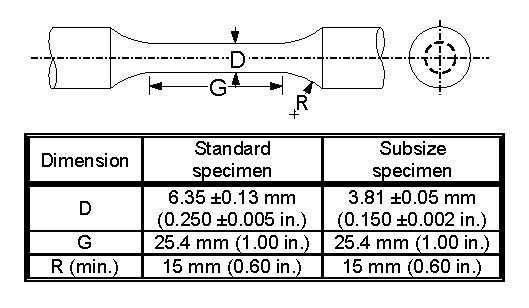
\includegraphics[width=.8\linewidth]{imgs/met/corpo_de_prova}
      \caption{Corpo de prova utilizado para o teste}
      \label{fig:corpo_de_prova}
    \end{subfigure}%
    \begin{subfigure}{.5\textwidth}
      \centering
      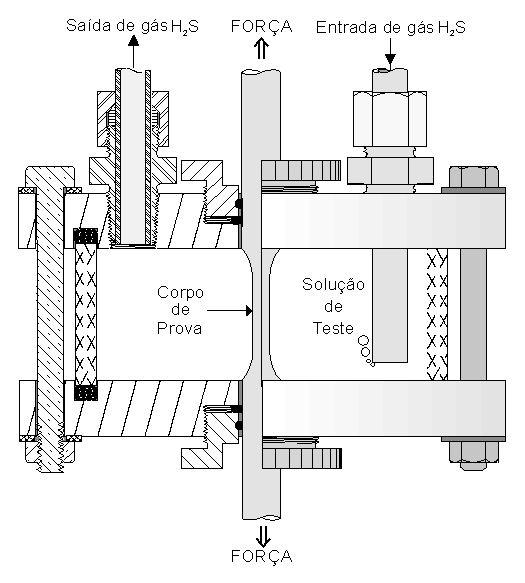
\includegraphics[width=.8\linewidth]{imgs/met/estrutura_de_teste}
      \caption{Esquemático da câmara para a realização do teste}
      \label{fig:sfig2}
    \end{subfigure}
    \legend{Fonte: NACE Standard TM0177 \cite[p. 7,8]{nace_standart} (Adaptada)}
    \label{fig:estrutura_de_teste}
    \end{figure}

O grande tempo despendido durante o teste e a necessidade de aguardar o resultado para prosseguir para as etapas seguintes de produção resulta em aumento de estoques e altos tempos para o atendimento dos pedidos dos clientes (lead time).

Diversas características que podem influenciar no resultado do teste foram levantadas e objetiva-se a determinação daquelas com maior significância para a determinação de um modelo capaz de realizar predições do resultado do teste.

\subsection{Descrição do Conjunto de dados}

Utilizando-se o conhecimento a priori do processo, uma filtragem inicial dos dados foi realizada, removendo caracteristicas irrelevantes para o processo de modelagem, tais como identificações, lotes e datas. Variáveis que não apresentam nenhuma variação no conjunto de dados também foram removidas. Além disso, por motivos de confidencialidade, o nome das variáveis foram anonimizados. Por fim, os dados passaram pelo processo de normalização descrito anteriormente.

Após o processamento inicial, o conjunto de dados possui 1064 amostras, com 30 possíveis variáveis de entrada e 3 varíaveis de saída.

